\chapter{Design Space Exploration}
\label{sec:dse}

In this section, we outline guidelines for  DSE over co-models of CPSs that: (a) support decision management by helping engineers to articulate clearly the parameters, objectives and metrics of a DSE analysis (Section~\ref{sec:dse-sysml}); and (b) enable the tuning of DSE methods for given domains and systems of interest (Section~\ref{sec:dse-algorithms}).
%
%
%\section{Experiment variables}
%
%\fbox{introduce parameters, architectures and scenarios and how they differ}
%
%

%
%\section{Ranking of designs}
%
%\fbox{methods for ranking and how they differ}
%


\section{Guidelines for Designing DSE in SysML}
\label{sec:dse-sysml}
\label{sec:dse-linefollow}

\subsection{Rationale}

Designing DSE experiments can be complex and tied closely to the multi-model being analysed. The definitions guiding the DSE scripts should not just appear with no meaningful links to the any other artefacts in the \into\ Tool  chain. There are two main reasons for this, firstly there is no traceability back to the requirements from which we might understand why the various objectives (measures) were being evaluated or why they were included in the ranking definition.  Secondly, if DSE configurations are created manually for each new DSE experiment it is easy to imagine that the DSE analysis and ranking might not be consistent among the experiments.

Engineers need, therefore, to be able to model at an early stage of design how the experiments relate to the model architecture, and where possible trace from requirements to the analysis experiments. Here we describe the first step towards this vision: a SysML profile for modelling DSE experiments. The profile comprises five diagrams for defining \emph{parameters}, \emph{objectives} and \emph{rankings}.

We take the same approach to defining the SysML profile for DSE as that used to define the INTO-SysML profile.  A metamodel is defined (see Deliverable D3.2b~\cite{INTOCPSD3.2b}) and the collection of profile diagrams that implement this metamodel are defined in Deliverable D4.2c~\cite{INTOCPSD4.2c}.
% and a collection of profile diagrams in Section~\ref{sec:dse-sysml-profile}.

%
%MOVED TO D3.2b
%
%\subsection{Metamodel}
%\label{sec:dse-sysml-metamodel}
%\draftnote{The following diagrams will be updated before final review to better reflect the examples}
%
%The metamodel for the DSE SysML extensions is presented in three fragments (we use Fragmenta~\cite{Amalio&15} as in Deliverable D2.1a~\cite{INTOCPSD2.1a}). The first fragment, in Figure~\ref{fig:dse_mm_param}, shows the elements required for the \texttt{DSEParameterDiagram}. A single \texttt{DSEAnalysis} block is defined along with several \texttt{Parameters} and \texttt{ParameterConstraints}. Parameters have values and refers to Component Variables. ParameterConstraints have a defined predicate.
%
%\begin{figure}[htbp]
%	\centering
%	\includegraphics[width=0.9\textwidth]{figures/MM_DSE_Param}
%\caption{Metamodel for DSE Parameter Diagram elements}
%\label{fig:dse_mm_param}
%\end{figure}
%
%The \texttt{DSEObjectiveDiagram} elements are defined in Figure~\ref{fig:dse_mm_obj}.  A single \texttt{DSEAnalysis} block is defined, as in the \texttt{DSEParameterDiagram}. The objective diagram contains a collection of \texttt{Objectives} and \texttt{ObjectiveConstraints}. Objectives have a collection of \texttt{FlowPorts} that are related to the \texttt{FlowPorts} owned by component \texttt{BlockInstances} of the INTO-SysML profile. The profile dictates two specialisations of Objectives -- \texttt{ExternalScripts} which have an associated file name, and \texttt{InternalFunctions} which have a function type. ParameterConstraints have a defined predicate.
%
%\begin{figure}[htbp]
%	\centering
%	\includegraphics[width=0.9\textwidth]{figures/MM_DSE_Obj}
%\caption{Metamodel for DSE Objective Diagram elements}
%\label{fig:dse_mm_obj}
%\end{figure}
%
%The final metamodel fragment, in Figure~\ref{fig:dse_mm_rank}, shows the model elements of the \texttt{DSERankingDiagram}. This diagram also contains a \texttt{DSEAnalysis} block and a collection of \texttt{Ranking} blocks. At present only the \texttt{Pareto} ranking is supported, which contains several \texttt{ParetoValues} -- each with a direction.
%
%\begin{figure}[htbp]
%	\centering
%	\includegraphics[width=0.9\textwidth]{figures/MM_DSE_Ranking}
%\caption{Metamodel for DSE Ranking Diagram elements}
%\label{fig:dse_mm_rank}
%\end{figure}

%
% MOVED TO D4.2c
%

%\subsection{SysML Profile}
%\label{sec:dse-sysml-profile}
%\draftnote{The following diagrams will be updated before final review to better reflect the examples in the next section.}
%
%
%The metamodel of Section~\ref{sec:dse-sysml-metamodel} is implemented as a SysML profile -- \textbf{DSE-SysML}, here defined using UML profile diagrams. The DSE-SysML extension is organised around the following four groups: diagram, parameters, objectives and ranking.
%
%The \textbf{DSE-SysML} profile defines three kinds of diagrams: the Parameter Diagram (PD); the Objective Diagram (OD); and the Ranking Diagram (RD). As shown in Figure~\ref{fig:dse_prof_overview}, these diagram types extend UML Class and Object diagrams.
%
%
%\begin{figure}[htbp]
%	\centering
%	\includegraphics[width=0.7\textwidth]{figures/Profile_DSE_Diagram}
%\caption{Profile diagram outlining DSE Profile diagrams}
%\label{fig:dse_prof_overview}
%\end{figure}
%
%Figure~\ref{fig:dse_prof_param} presents the parameter group, which realises the ParameterDiagram metamodel fragment of Figure~\ref{fig:dse_mm_param}. This is based on specialising the INTO-SysML Block stereotype (which in turn extends the SysML Block stereotype, which extends the UML Class metaclass), which enables us to incorporate the metamodel elements of the fragment. The diagram states that a \texttt{DSEAnalysis} block may contain \texttt{Parameter} and \texttt{ParameterConstraint} blocks. Parameters contain \texttt{Variable} stereotypes extending the UML Property metaclass.
%
%
%\begin{figure}[htbp]
%	\centering
%	\includegraphics[width=0.8\textwidth]{figures/Profile_DSE_Param}
%\caption{Profile diagram for DSE Parameter Diagram elements}
%\label{fig:dse_prof_param}
%\end{figure}
%
%The objective group is shown in Figure~\ref{fig:dse_prof_obj}. Similar to the parameter group, a \texttt{DSEAnalysis} block may contain \texttt{Objectives} and \texttt{ObjectiveConstraints} -- all stereotypes extending the SysML Block stereotype. Objectives contain a collection of \texttt{FlowPorts} -- as defined in the INTO-SysML profile.
%
%\begin{figure}[htbp]
%	\centering
%	\includegraphics[width=0.85\textwidth]{figures/Profile_DSE_Obj}
%\caption{Profile diagram for DSE Objective Diagram elements}
%\label{fig:dse_prof_obj}
%\end{figure}
%
%The final group, ranking, is defined in Figure~\ref{fig:dse_prof_rank}. Again, extending the INTO-CPS Block stereotype, the \texttt{DSEAnalysis} element contains a single \texttt{Ranking} object (this stereotype also extends the INTO-SysML Block stereotype). The Ranking element is extended by the \texttt{Pareto} stereotype.
%
%\begin{figure}[htbp]
%	\centering
%	\includegraphics[width=0.5\textwidth]{figures/Profile_DSE_Rank}
%	\caption{Profile diagram for DSE Ranking Diagram elements}
%\label{fig:dse_prof_rank}
%\end{figure}
%
%\section{Line Follow Robot SysML Example}
%\label{sec:dse-linefollow}

In this section, we present an illustrative example of the use of the DSE-SysML profile -- from requirements engineering through defining parameters and objectives in the DSE-SysML profile to the final DSE JSON configuration files. We present result of the execution of DSE for the defined configuration.

As an example, we use the line follower robot pilot study. More details can be found in Deliverable D3.5~\cite{INTOCPSD3.5}.

\subsection{Requirements}

We propose the use of a subset of the SoS-ACRE method detailed in Chapter~\ref{sec:reqeng} (as this section concentrates on the application of the DSE-SysML profile, we don't consider the full SoS-ACRE process). In the Requirements Definition View in Figure~\ref{fig:line_rdv}, the following five requirements are defined:

\begin{enumerate}
	\item The robot shall have a minimal cross track error
	\item The cross track error shall never exceed \textbf{X} mm
	%\item The robot shall maximise its potential range
	%\item The robot shall have a minimal range of \textbf{X} m
	\item The robot shall maximise its average speed
	\item The robot shall have a minimum average speed of \textbf{X} ms$^{-1}$
%	\item The robot shall maximise its operating time between battery charges
%	\item The robot shall have a minimum operating time of \textbf{X}s
	\item The robot sensor positions may be altered to achieve global goals
\end{enumerate}

\begin{figure}[htbp]
	\centering
	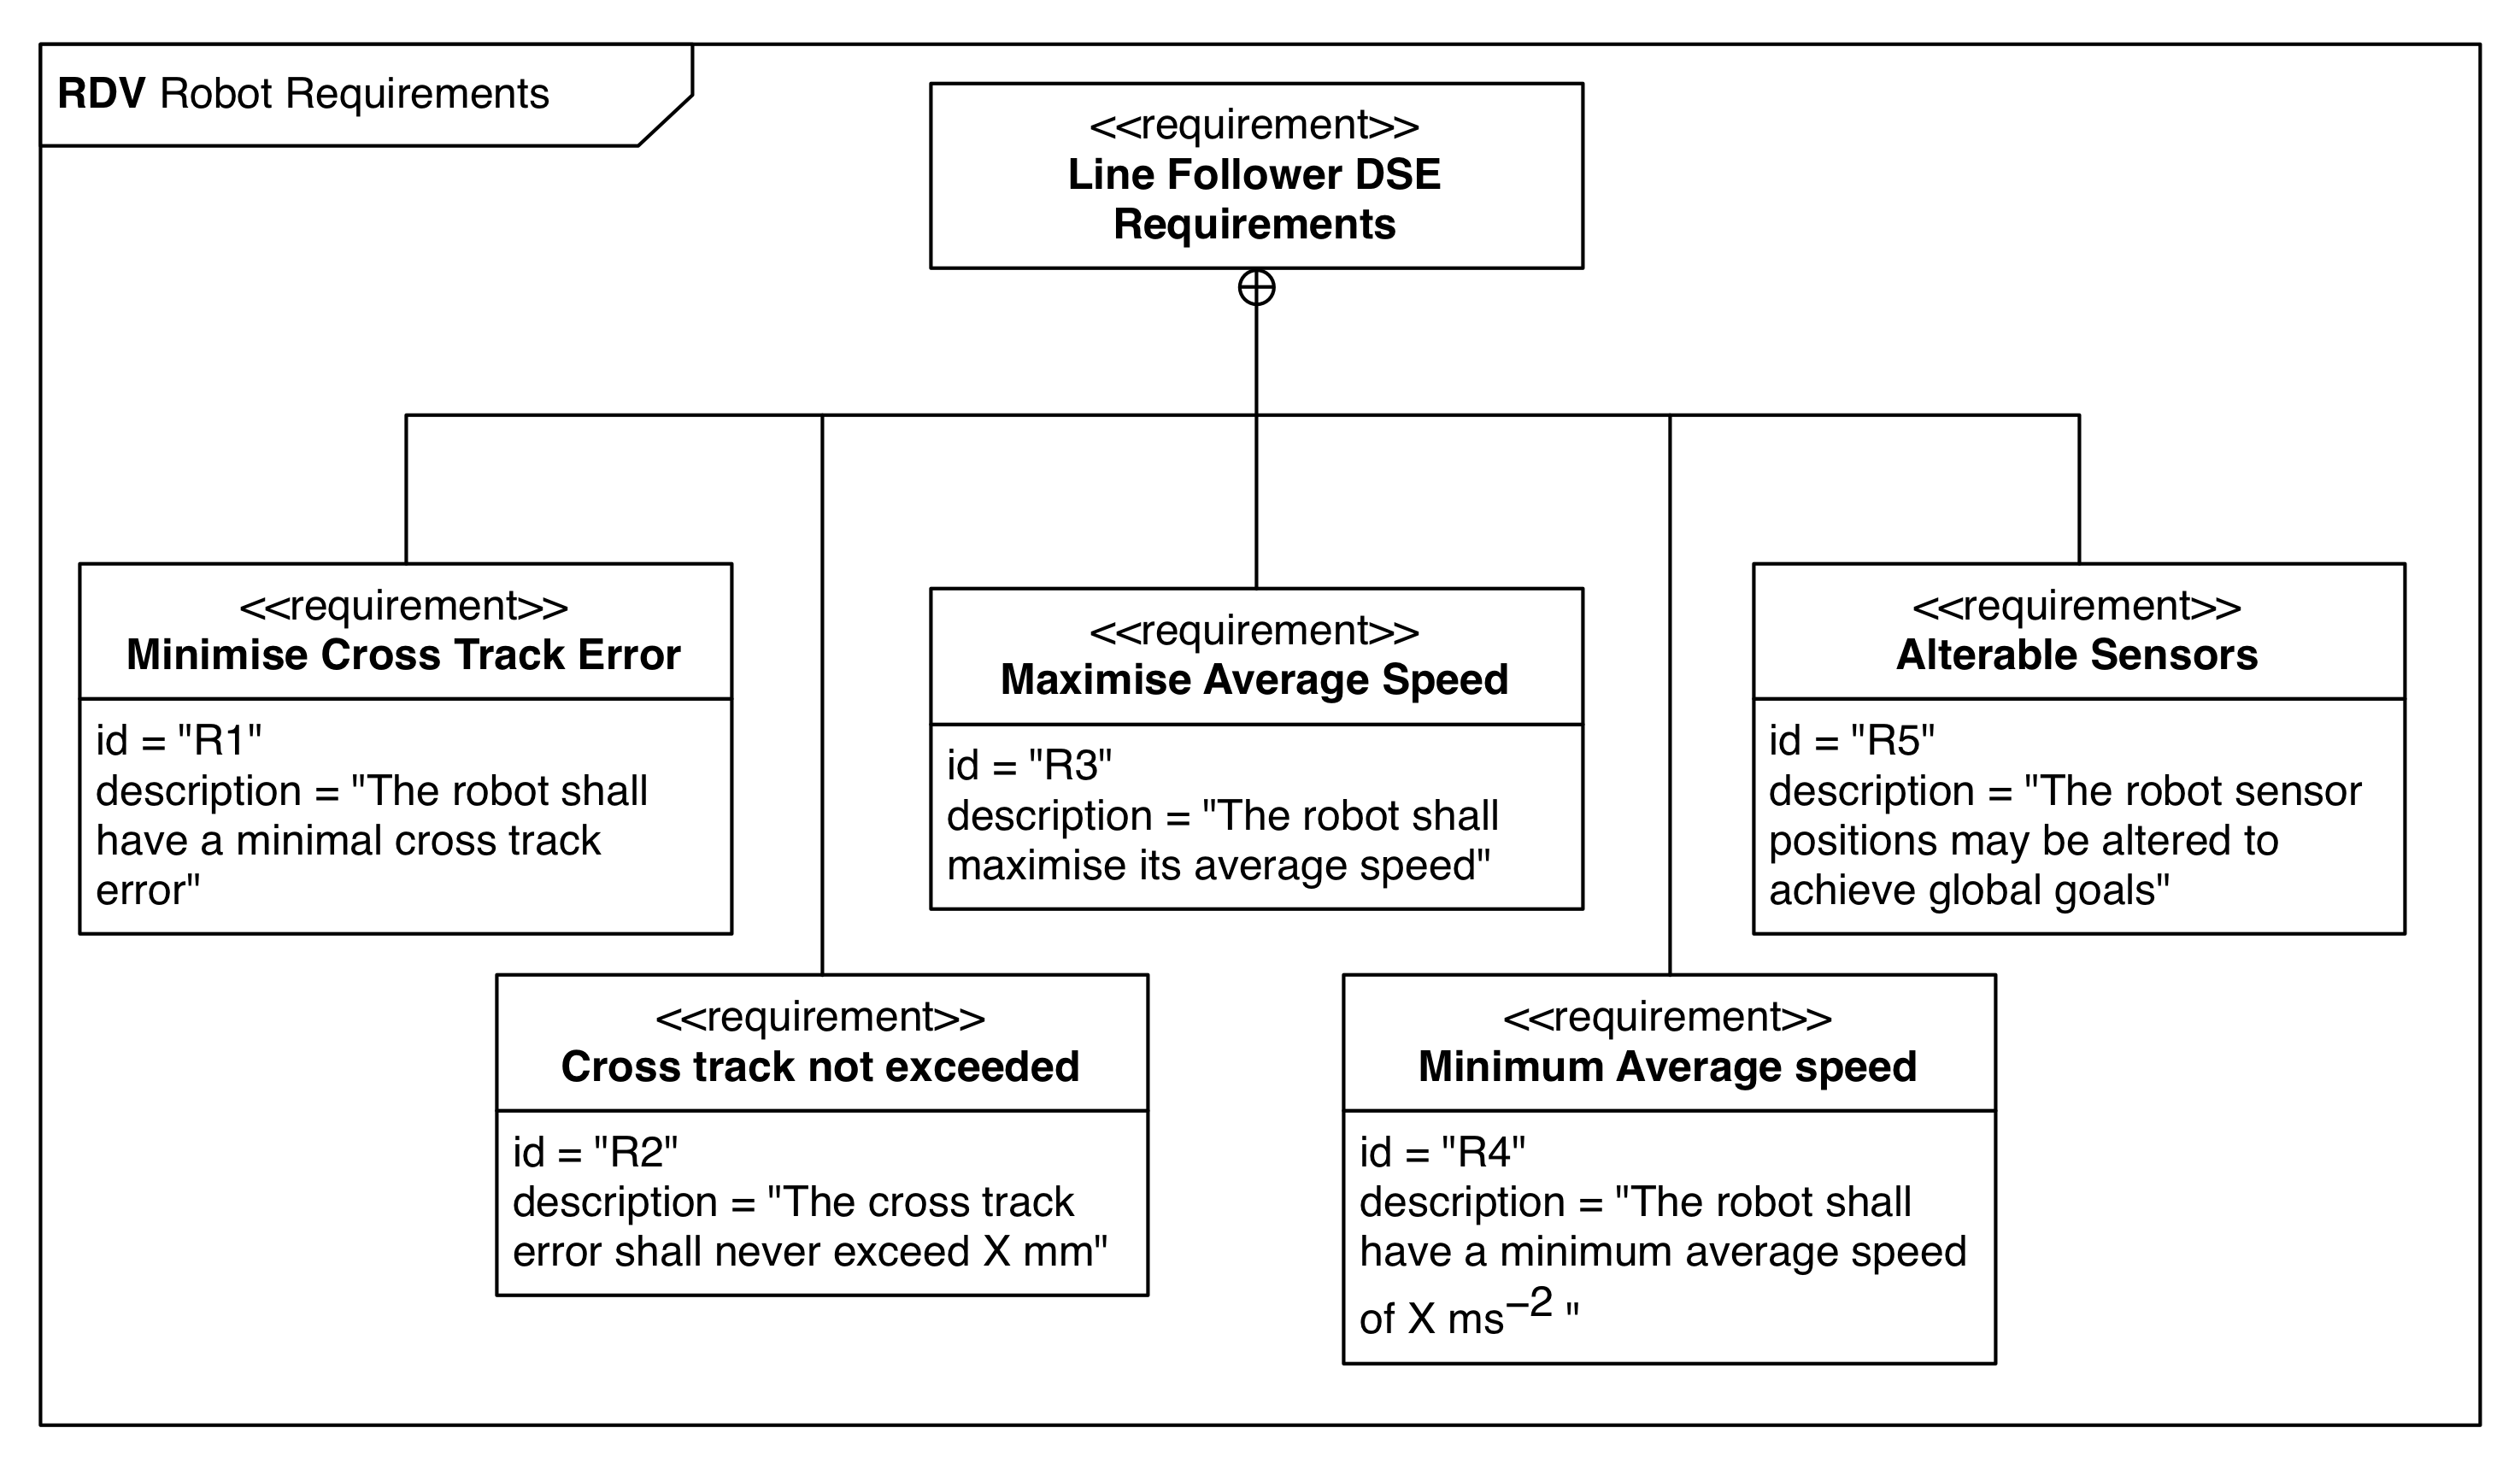
\includegraphics[width=0.8\textwidth]{figures/Robot_RDV}
\caption{Subset of the Requirements Definition View for requirements of the Line Following Robot}\label{fig:line_rdv}
\end{figure}


%\draftnote{Use appropriate requirements diagrams here}

\subsection{Objectives from Requirements}

Based upon the requirements above, we define two objectives: the calculation of deviation from a desired path, and the speed of the robot.

\paragraph{Deviation}

The deviation from a desired path, referred to as the cross track error, is the distance the robot moves from the line of the map, as shown in Figure~\ref{fig:crossTrackError}.

\begin{figure}[htbp]
	\centering
	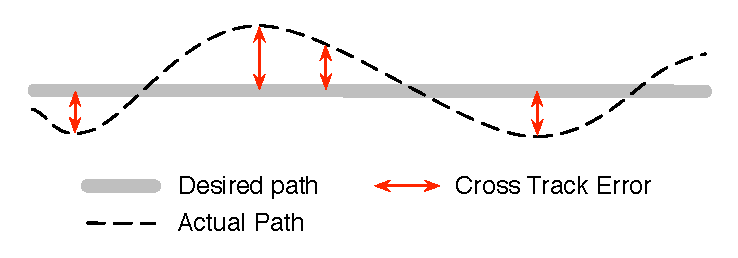
\includegraphics[scale=0.8]{figures/crossTrackError}
\caption{Cross track error at various points for a robot trying to follow a desired line}\label{fig:crossTrackError}
\end{figure}

To compute cross track error we need some model of the desired path to be followed and the actual path taken by the robot.  Each point on the actual path is compared with the model of the desired path to find its distance from the closest point, this becomes the cross track error.  If the desired path is modelled as a series of points, then it may be necessary to find shortest distance to the line between the two closest points.


%\paragraph{Range}



\paragraph{Speed}
The speed may be measured in several ways depending on what data is logged by the COE and what we really mean by speed, indicated in Figure~\ref{fig:robotSpeed}.

\begin{figure}[htbp]
	\centering
	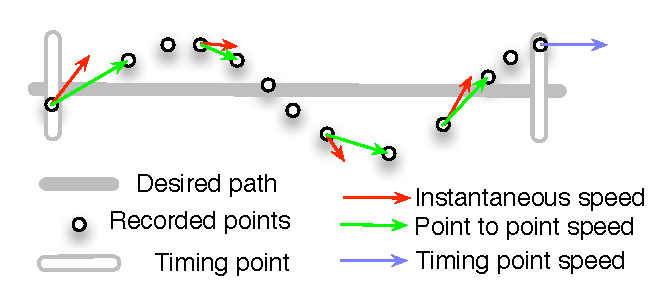
\includegraphics[scale=0.8]{figures/robotSpeed}
\caption{Cross track error at various points for a robot trying to follow a desired line}\label{fig:robotSpeed}
\end{figure}

Inside the CT model there is a bond graph flow variable that represents the forwards motion of the robot.  This variable is not currently logged by the COE but it could be and this would result in snapshots of the robot speed being taken when simulation models synchronise.  In this example, we take the view that speed is referring to the time taken to complete a lap.

%\paragraph{Longevity}

\subsection{SysML Representation of Parameters, Objectives and Ranking}

We next consider the use of the upcoming DSE profile to define the DSE parameters, objectives and desired ranking function. In the following SysML diagrams, we explicitly refer to model elements as defined in the architectural model of the line follower study, presented in Deliverable D3.5~\cite{INTOCPSD3.5}.

\paragraph{Parameters}   In the requirements defined above, we see that the position of the line follower sensors may be varied. In real requirements, we may elicit the possible variables allowed. Figure~\ref{fig:dse_lfr_param} is a DSE Parameter Definition Diagram and defines four parameters required: \emph{S1\_X}, \emph{S1\_Y}, \emph{S2\_X} and \emph{S2\_Y}, each a set of real numbers.  The DSE experiment in this example is called \emph{DSE\_Example}.

\begin{figure}[htbp]
	\centering
	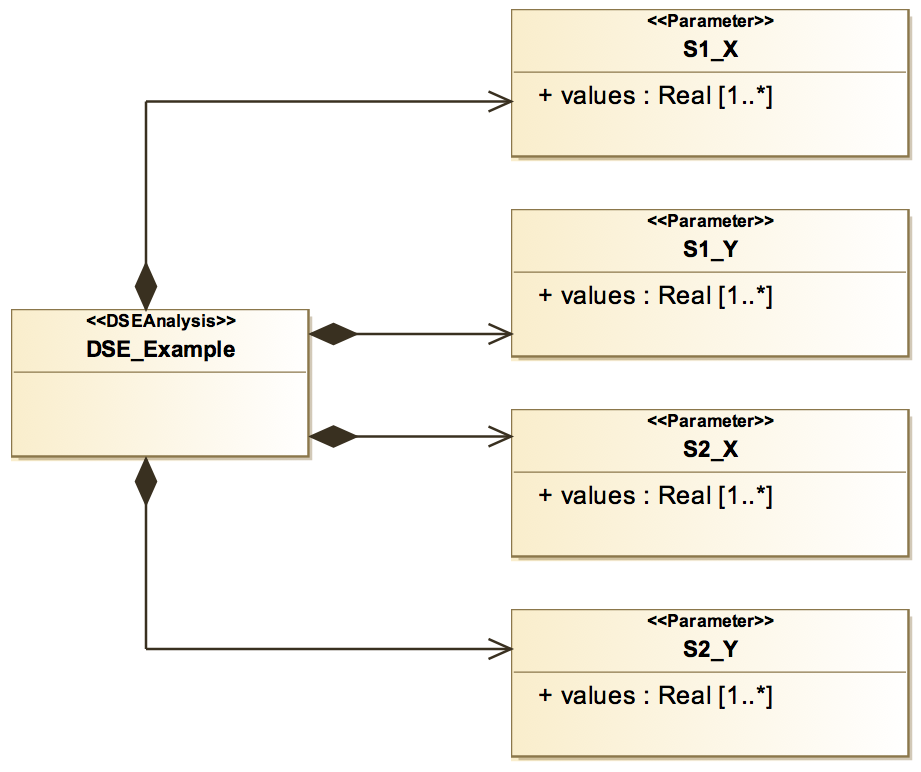
\includegraphics[width=0.7\textwidth]{figures/LFR_DSE_Param}
\caption{DSE-SysML Parameter Definition Diagram of Line Following Robot example}
\label{fig:dse_lfr_param}
\end{figure}

Figure~\ref{fig:dse_lfr_param2} identifies the architectural model elements themselves (the \texttt{lf\_position\_x} and  \texttt{lf\_position\_y} parameters of \emph{sensor1} and  \emph{sensor2}) and the possible values each may have (for example the \texttt{lf\_position\_x} parameter of \emph{sensor1} may be either $0.01$ or $0.03$). The diagram (or collection of diagrams if there is a large number of design parameters) should record all parameters for the experiment.

\begin{figure}[htbp]
	\centering
	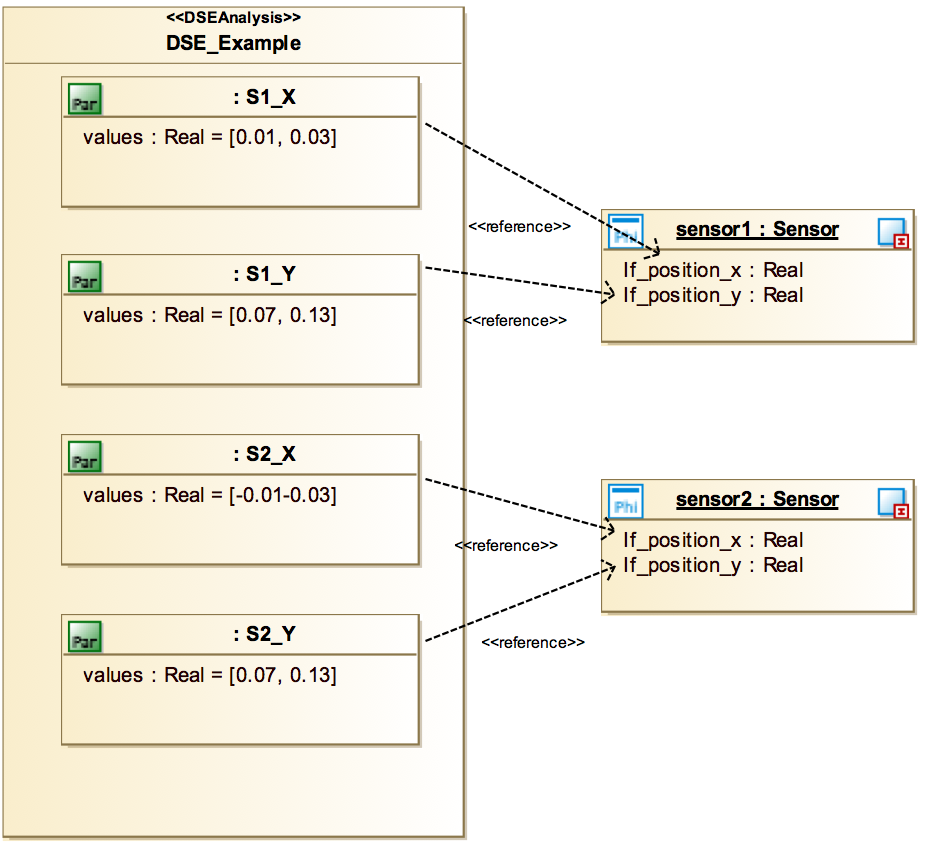
\includegraphics[width=0.7\textwidth]{figures/LFR_DSE_Param2}
\caption{DSE-SysML Parameter Connection Diagram of Line Following Robot example}
\label{fig:dse_lfr_param2}
\end{figure}

\paragraph{Objectives}    The objectives follow from the requirements as mentioned above. Figure~\ref{fig:dse_lfr_obj} shows the DSE Objectives Definition Diagram with four objectives:  \emph{meanSpeed}, \emph{lapTime}, \emph{maxCrossTrackError} and \emph{meanCrossTrackError}. Each have a collection of inputs -- defined either as constants (e.g. parameter \emph{p1} of \emph{meanSpeed}), or to be obtained for the multi-model.

\begin{figure}[htbp]
	\centering
	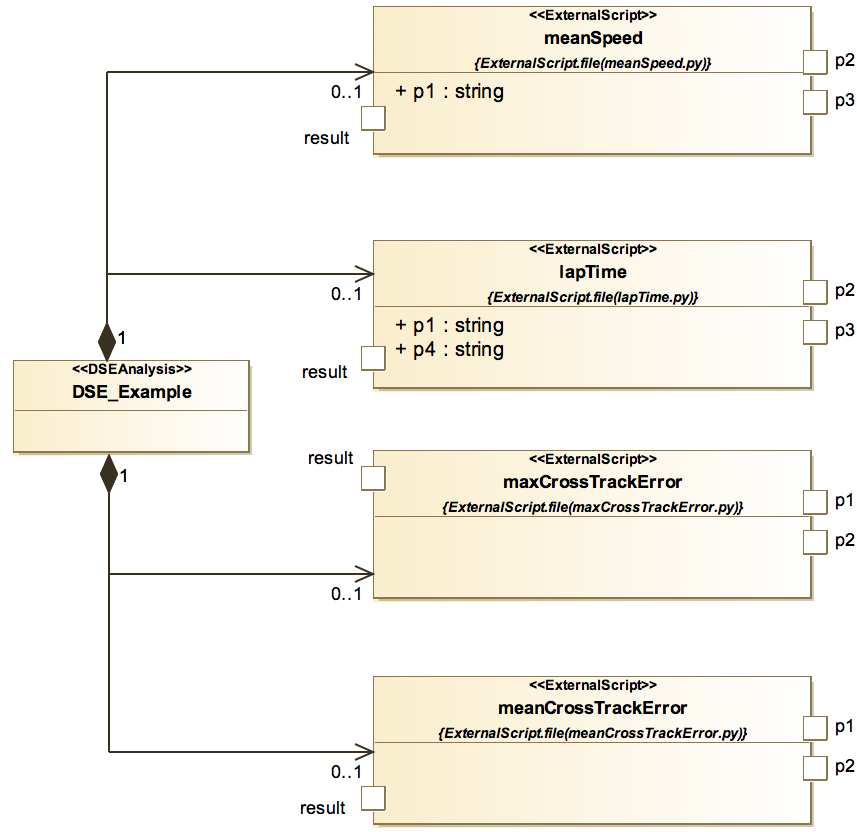
\includegraphics[width=0.7\textwidth]{figures/LFR_DSE_Obj}
\caption{DSE-SysML Objective Definition Diagram of Line Following Robot example}
\label{fig:dse_lfr_obj}
\end{figure}

The objective definitions are realised in Figure~\ref{fig:dse_lfr_obj2}. The \emph{meanSpeed} requires the step-size of the simulation (this is obtained from the co-simulation results, rather than defined here) and the \texttt{robot\_x} and \texttt{robot\_y} position of the robot body. The \emph{lapTime} objective requires the time at each simulation step (again, obtained directly from the co-simulation output), the \texttt{robot\_x} and \texttt{robot\_y} position of the robot body and the name of the map. Both the \emph{maxCrossTrackError} and \emph{meanCrossTrackError} objectives require only the \texttt{robot\_x} and \texttt{robot\_y} position of the robot body.

\begin{figure}[htbp]
	\centering
	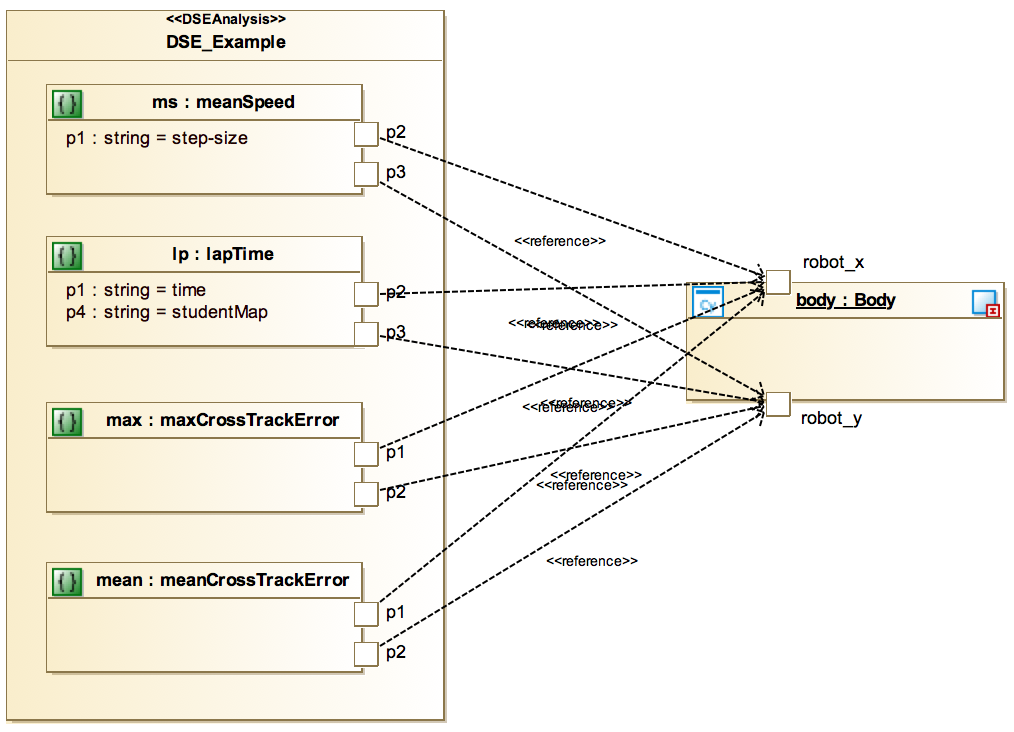
\includegraphics[width=0.7\textwidth]{figures/LFR_DSE_Obj2}
\caption{DSE-SysML Connection Objective Diagram of Line Following Robot example}
\label{fig:dse_lfr_obj2}
\end{figure}

\paragraph{Ranking} Finally, the DSE Ranking Diagram in Figure~\ref{fig:dse_lfr_rank} defines the ranking to be used in the experiment. This diagram states that the experiment uses the Pareto method, and is a 2-value Pareto referring to the \emph{lapTime} and \emph{meanCrossTrackError} objectives.

\begin{figure}[htbp]
	\centering
	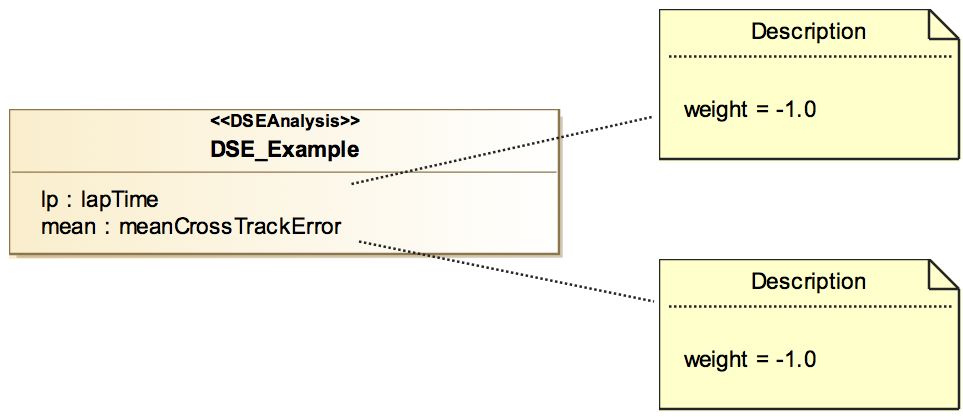
\includegraphics[width=0.6\textwidth]{figures/LFR_DSE_Rank}
\caption{Example DSE-SysML Ranking Diagram of Line Following Robot example}
\label{fig:dse_lfr_rank}
\end{figure}

\subsection{DSE script}

\draftnote{TWT: Please update this paragraph. Is this Modelio export available now?}

These diagrams may then be translated to the JSON config format required by the DSE tool (see the INTO-CPS User Manual, Deliverable D4.2a~\cite{INTOCPSD4.2a} for more details). At present this is a manual process, however tool support in Modelio is in preparation and shall be available early in Year 3 of the project. This tool support will provide the automated generation of a skeleton configuration, specifying the parameters, objectives and ranking to use. This leaves the choice of DSE algorithm and simulation timing settings for an engineer to specify in the INTO-CPS application.
Figure~\ref{fig:dse_config_json} shows the corresponding DSE configuration file for the line follower experiments. Note that where we refer to model elements of the architecture (such as model parameters), we now use the same conventions used in the co-simulation orchestration engine configuration.

\begin{figure}[h]
	\centering
	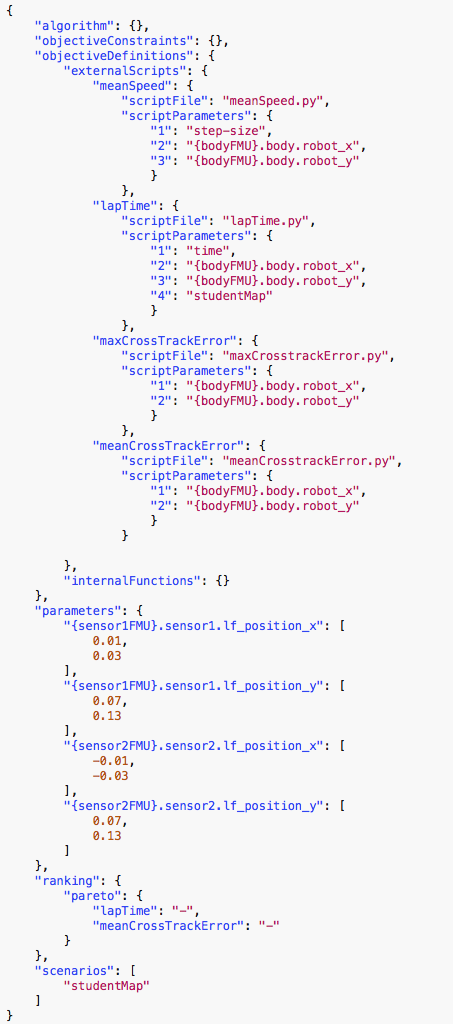
\includegraphics[scale=0.45]{figures/config-whole}
		\caption{A complete DSE configuration JSON file for the line follower robot example}
		\label{fig:dse_config_json}
\end{figure}

\subsection{DSE results}

DSE is performed in the DSE tool (again, see the INTO-CPS User Manual, Deliverable D4.3a~\cite{INTOCPSD4.3a} for more detail) by processing the DSE configuration using scripts that contain the required algorithms.  The main scripts contain the search algorithm that determines which parameters to use in each simulation, the simplest of these is the exhaustive algorithm that methodically runs through all combinations of parameters and runs a simulation of each.  The log files produced by each simulation are then processed by other scripts to obtain the objective values defined in the previous section.  Finally, the objective values are used by a ranking script to place all the simulation results into a partial order according to the defined ranking.  The ranking information is used to produce tabular and graphical results that may be used to support decisions regarding design choices and directions.

Figure~\ref{fig:dse-results} shows an example of the DSE results from the line follower robot where the lap time and mean cross track error were the objectives to optimise.  These results contain two representations of the data, a graph plotting the objective values for each design, with the Pareto front of optimal trade-offs between the key objectives highlighted, here in blue. The second part of the results presents the data is tables, indexed by the ranking position of each result.  This permits the user to determine the precise values for both the measured objectives and also the design parameters used to obtain that result.

\begin{figure}[h!]
	\centering
	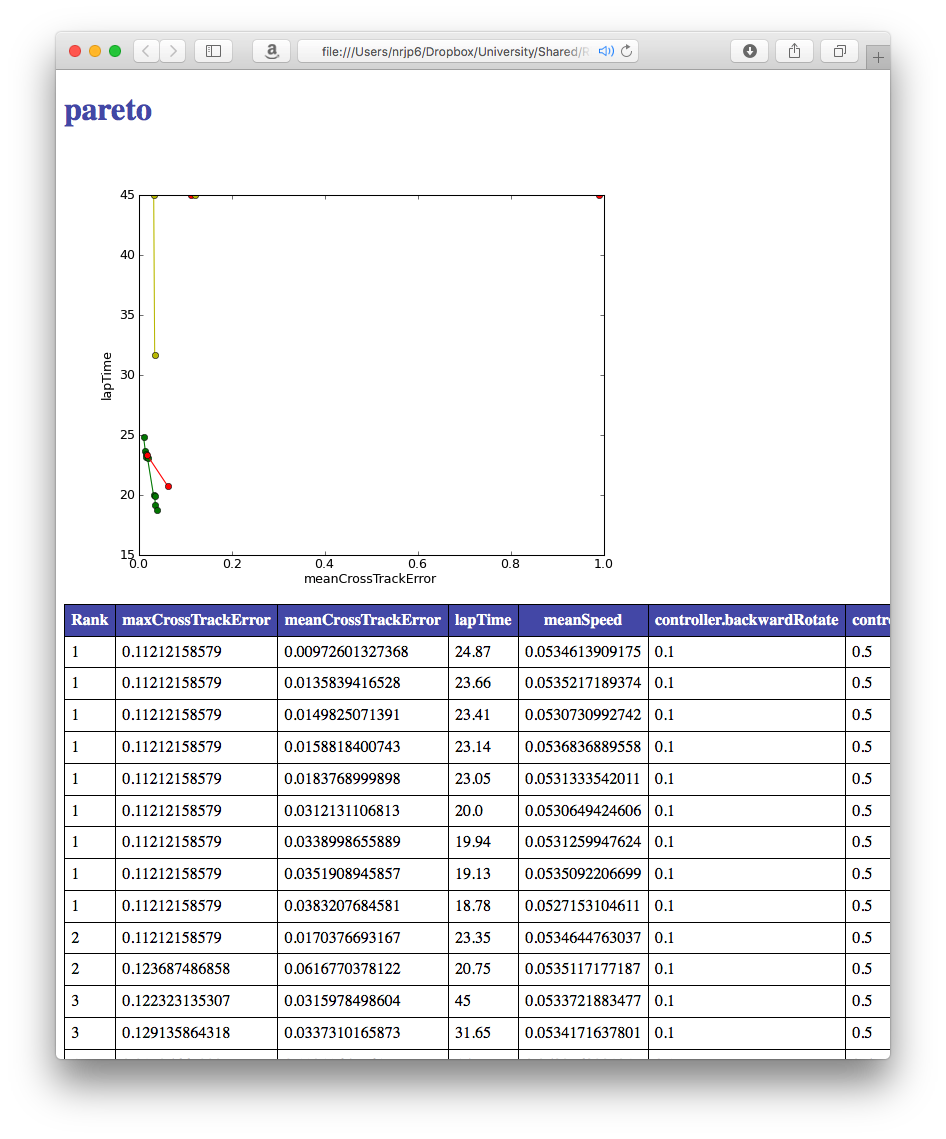
\includegraphics[width=0.9\textwidth]{figures/dse_results}
	\caption{DSE results}
	\label{fig:dse-results}
\end{figure}

\section{An Approach to Effective DSE}
\label{sec:dse-algorithms}

Given a ``designed'' design space using the method detailed above, we use the INTO-CPS Tool Chain to simulate each design alternative. The initial approach we took was to implement an algorithm to exhaustively search the design space, and evaluate and rank each design. Whilst this approach is acceptable on small-scale studies, this quickly becomes infeasible as the design space grows. For example, varying $n$ parameters with $m$ alternative values produces a design space of $m^n$ alternatives. In the remainder of this paper, we present an alternative approach to exploring the design space in order to provide guidance for CPS engineers on how to design the exploration of designs for different classes of problems.

\subsection{A Genetic Algorithm for DSE}
Inspired by processes found in nature, genetic algorithms ``breed'' new generations of optimal CPS designs from the previous generation's best candidates. This mimics the concept of survival of the fittest in Darwinian evolution.
Figure~\ref{fig:ga_dse_process} represents the structure of a genetic algorithm used for DSE.  Several activities are reused from exhaustive DSE: simulation; evaluation of objectives; rank simulated designs; and generate results. The remaining activities are specific to the genetic approach and are detailed in this section.

\begin{figure}[h!]
	\centering
	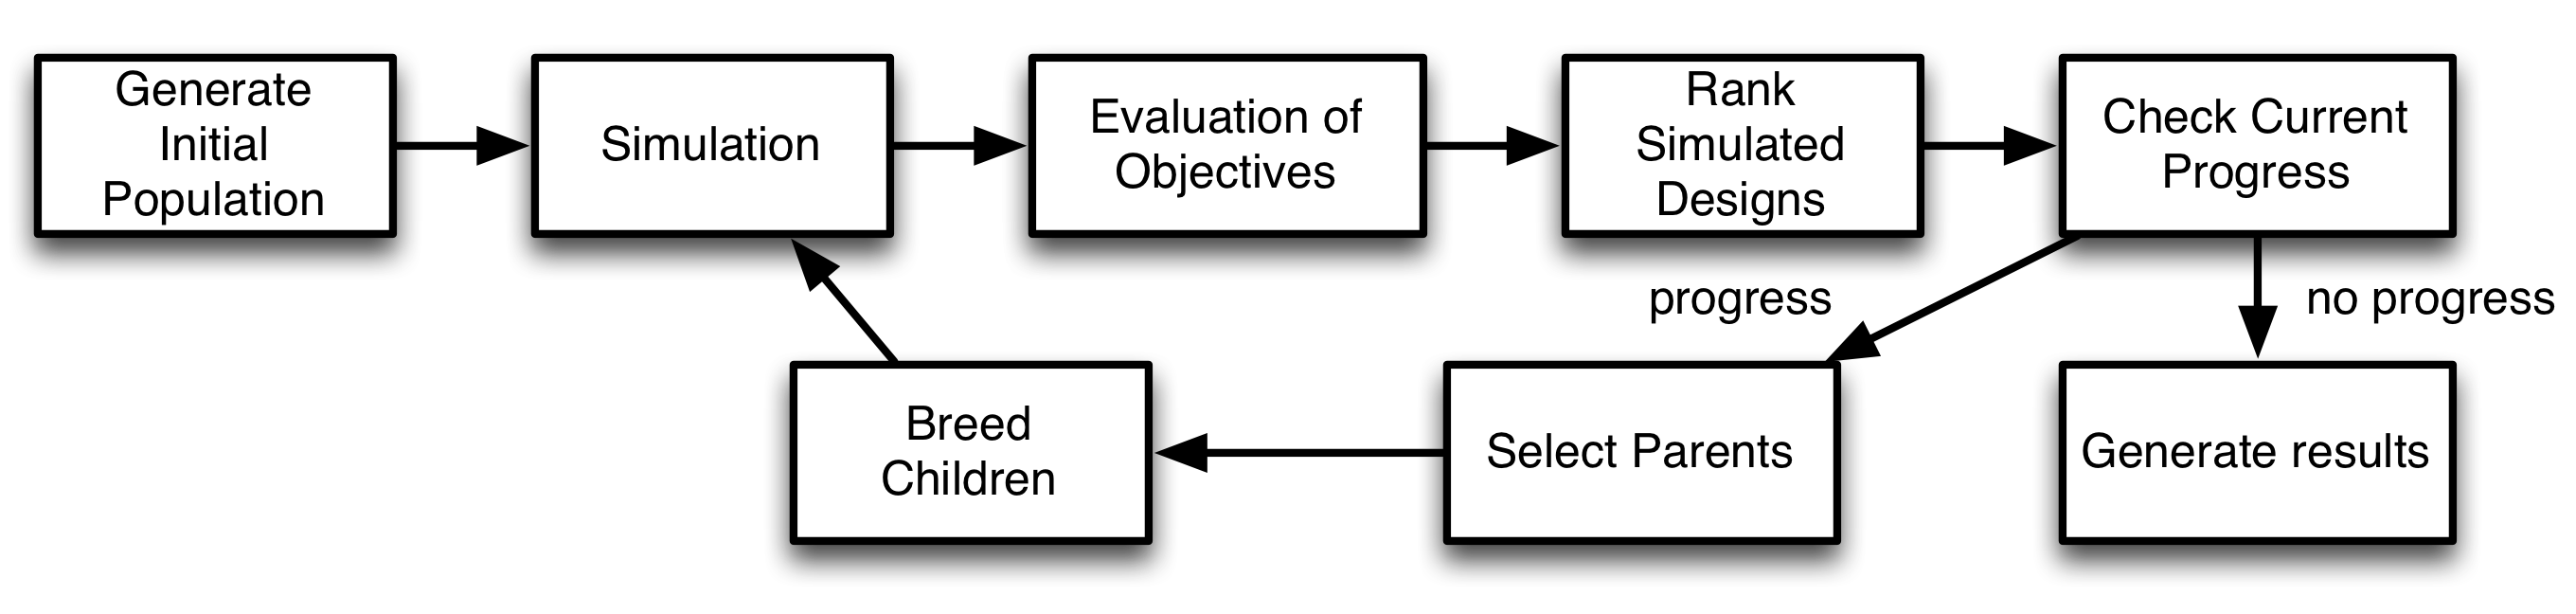
\includegraphics[width=0.9\textwidth]{figures/ga_process}
	\caption{High-level process for DSE Genetic Algorithm}
	\label{fig:ga_dse_process}
\end{figure}

\begin{description}
\item[Generating initial population:] Two methods for generating an initial population of designs are supported: randomly, or uniformly across the design space. Generating an initial design set which is distributed uniformly could allow parts of the design space to be explored that would otherwise not be explored with a random initial set. This could give us greater confidence that the optimal designs found by the genetic algorithm are consistent with the optimal designs of the total design space.
\item[Selecting parents:] Two options for parent selection are supported: random and distributed. Random selection means that two parents are chosen randomly from the non-dominated set (NDS). There is also a chance for parents to be selected which are not in the NDS, potentially allowing different parts of the design space to be explored due to a greater variety of children being produced.

\draftnote{AI: Maybe we should put NDS in the glossary list}

An intelligent approach involves calculating the distribution of each design's objectives from other designs in the NDS. One of the parents chosen is the design with the greatest distribution, enabling us to explore another part of the design space which may contain other optimal designs. Picking a parent that has the least distribution suggests that this parent is close to other optimal designs, meaning that perhaps it is likelier to produce optimal designs.
		
Figure~\ref{fig:ga_fitness} shows the fitness roulette by which how much a design solution in Figure~\ref{fig:ga_fitness2} satisfies the requirements. It can be seen that there exists a relationship where the greater the fitness value a design has, the more likely it is to be selected as a parent. The probability $P$ of design d being selected as a parent can be calculated by:

\begin{figure}[htbp]
\begin{center}
\subfigure[Example fitness roulette]
{
	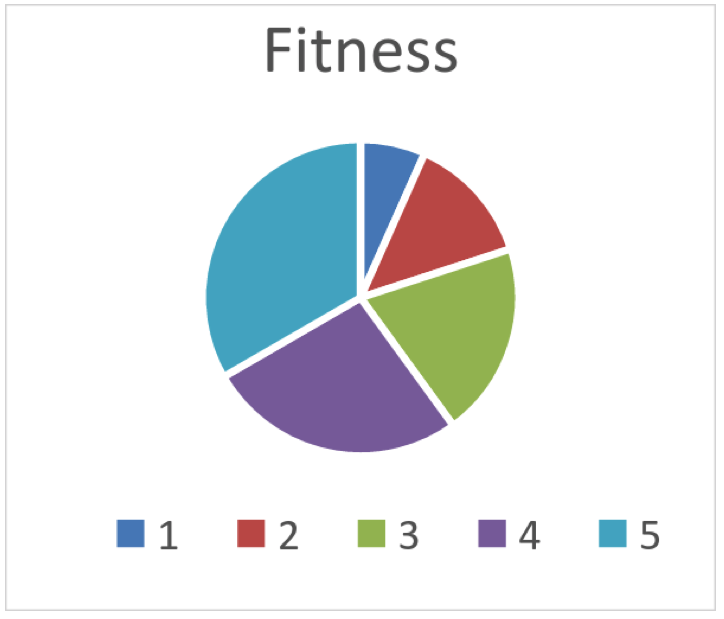
\includegraphics[width=0.25\textwidth]{figures/ga_fitness}
	\label{fig:ga_fitness}
}
\subfigure[Fitness of designs]
{
	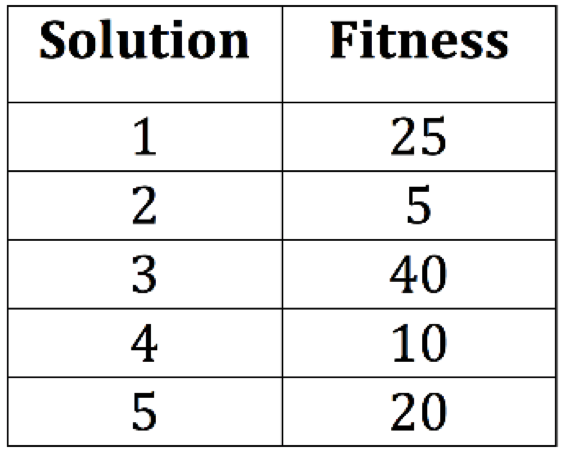
\includegraphics[width=0.25\textwidth]{figures/ga_fitness2}
	\label{fig:ga_fitness2}
}
\caption{Genetic Algorithm fitness selection}
\label{fig:ga_fitness_all}
\end{center}
\end{figure}


\item[Breeding children:] After the parents are selected, the algorithm creates two new children using a process of crossover. Figure~\ref{fig:ga_crossover} shows this process. Mutation could also occur, where a randomly chosen parameter's value is replaced by another value defined in the initial DSE configuration, producing new designs to explore other parts of the design space.

\begin{figure}[h!]
	\centering
	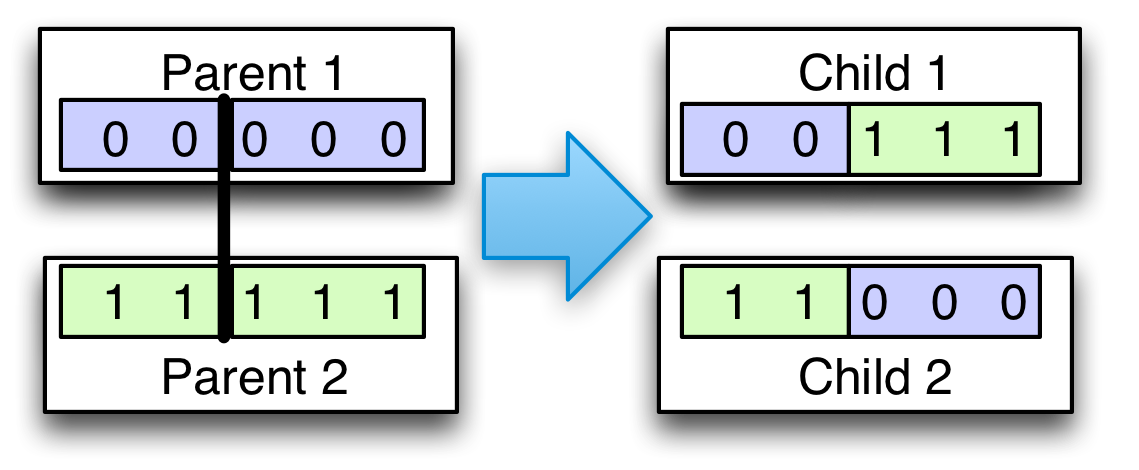
\includegraphics[width=0.45\textwidth]{figures/ga_breeding}
	\caption{Depiction of genetic crossover}
	\label{fig:ga_crossover}
\end{figure}

\item[Checking current progress:] Progression is determined by the change in the NDS on each iteration. It is possible to tune the number of iterations without progress before termination.

\end{description}
\subsection{Measuring Effectiveness}
To provide guidance on selection and tuning of a specific algorithm to a DSE situation it is necessary that there is a means for experimenting with the algorithm parameters and also means for evaluating the resulting performance. To this end an experiment was devised that supports exploration of these parameters using a range of design spaces as the subject.
The experiment is based upon generating a ground truth for a set of design spaces such that the composition of each Pareto front is known and we may assess the cost and accuracy of the genetic algorithm's attempt to reach it. A limiting factor for these design spaces is that they must be exhaustively searched and so there are current four of these all based upon the line follow robot: an 81-point and a 625-point design space where the sensor positions are varied and a 216-point and 891-point design spaces where the controller parameters are varied.
There are three measures applied to each result that target the tension between trading off the cost of running a DSE against the accuracy of the result

\begin{description}
\item[Cost:] The simplest of the measures is the cost of the performing the search and here it is measured by the number of simulations performed to reach a result. For the purposes of comparison across the different design spaces, this cost is represented as a proportion of the total number of designs

$cost = \frac{|Simulations\ Run|}{|Design\ Space|}$

\item[Accuracy:] The ground truth exhaustive experiments provide us with the Pareto Front for that design space and each DSE experiment returns a non-dominated set of best designs found.  Here the accuracy measure considers how many of the designs in the genetic non-dominated set are actually the best designs possible. It is measured by finding the proportion of points in the genetic NDS that are also found in the ground truth Pareto front.

$accuracy = \frac{|GeneticNDS \cap ExhaustiveNDS|}{|GeneticNDS|}$

\item[Generational Distance:] The accuracy measure tells us something about the points in the genetically found NDS that are also found in the exhaustive NDS (Van Veldhuizen \& Lamont, 2000).  The generational distance gives us a figure indicating the total distance between the genetic NDS and the exhaustive NDS. It is calculated by computing the sum of the distance between each point in the genetic NDS and its closest point in the exhaustive NDS and dividing this by the total number of points.


$generational\ distance = \frac{\sqrt{(\sum_{i=1}^{n} d_{i}^{2})}}{n}$

\end{description}
\subsection{Genetic DSE Experiments and Results}
The DSE experiments involved varying three parameters of the genetic algorithm and repeating each set of parameters with each design space five times.  The parameters of the genetic algorithm varied were:

\begin{description}
\item[Initial population size:] The initial population size took one of three values.  All design spaces were tested using an initial population of 10 designs, they were also tested with initial populations equal to $10\%$ of the design space and $25\%$ of the design space.  These are represented on the left hand graphs by the $10$, $10\%$ and $25\%$ lines.
\item[Progress check conditions:] The number of rounds the genetic algorithm would continue if there was no progress observed was tested with three values, 1, 5 and 10.  These are represented on the right hand graphs with the 1, 5 and 10 lines.

\item[Algorithm options:] There are two variants of the genetic algorithm, phase 1 with random initial population and random parent selection, and phase 3 which give an initial population distributed over the design space and where parent selection is weighted to favour diverse parents.  The phase one experiments are on the left hand side of the graphs, with points labelled `<design space size>-p1' while the phase three experiments are on the right labelled `<design space size>-p3'.
\end{description}

The results of the simulations are shown in graph form below.  Each point graphed is the averaged result of the five runs of each set of parameters.  Figure~\ref{fig:cost_ga_ex}, shows the graphs of cost of running the DSEs.  Encouragingly there is a slight trend of the cost of DSE reducing as a proportion of the design space as the design space size increases.  As expected the cost was greater with larger initial populations but the cost did not vary when changing the progress check condition as much as expected.

\begin{figure}[p]
	\centering
	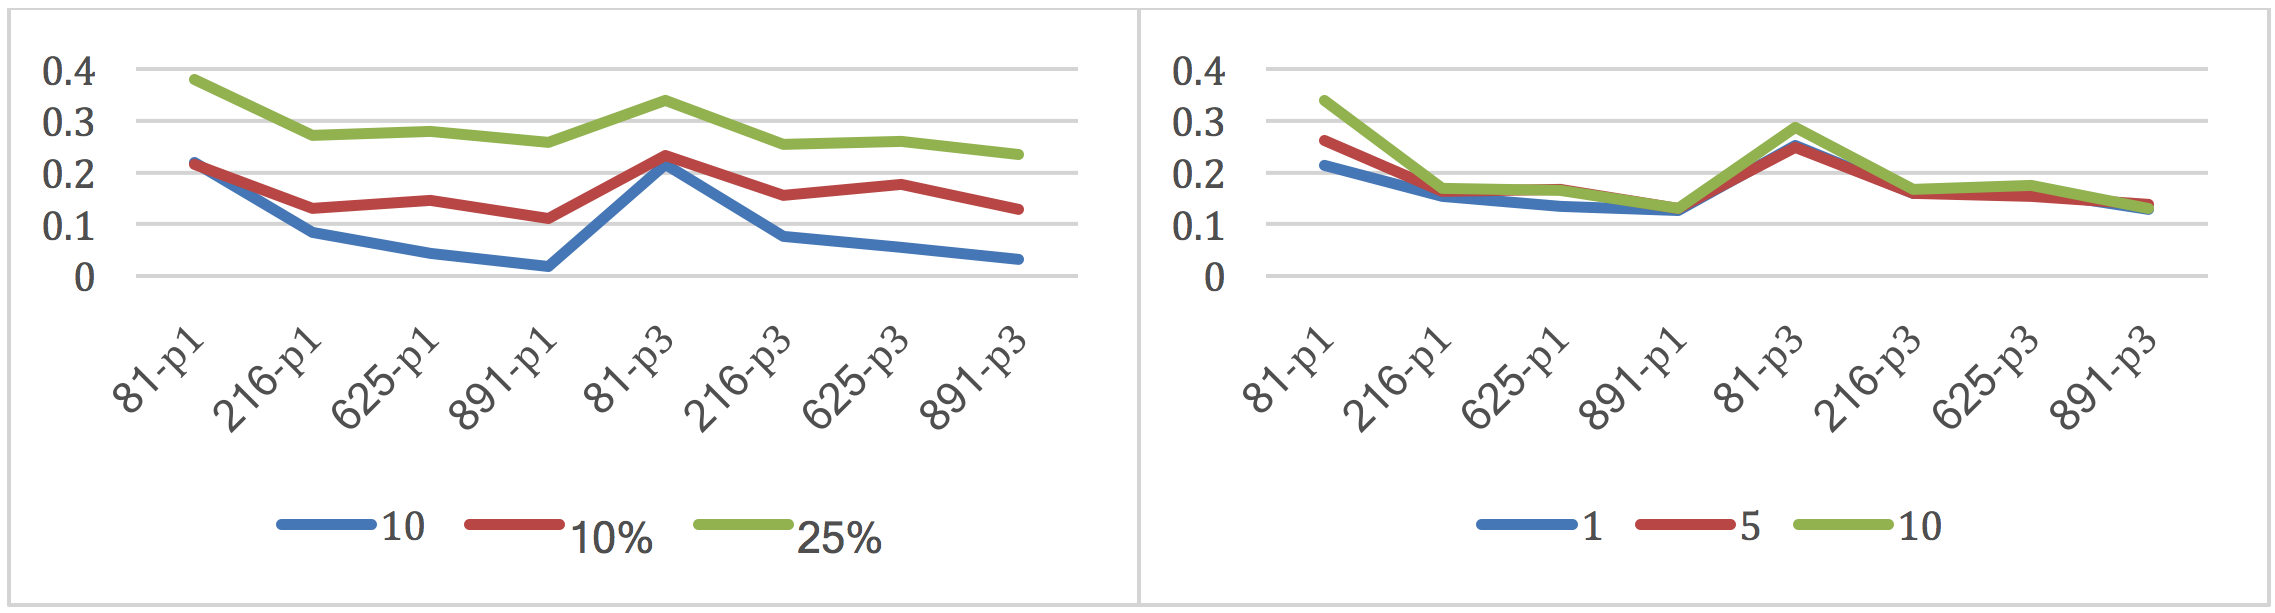
\includegraphics[width=1\textwidth]{figures/ga_cost}
	\caption{Cost of DSE, number of simulations run as proportion of the total design space}
	\label{fig:cost_ga_ex}
\end{figure}
Figure~\ref{fig:acc_ga_ex} shows the graphs of DSE accuracy.  There is again a slight downward trend as design space size increases, meaning that there is a slight increase in the number of points in the genetic NDS that are not truly optimal.  As expected the larger initial population generally resulted in more accurate NDS, this was also true of using the largest value for the progress check condition.

\begin{figure}[p]
	\centering
	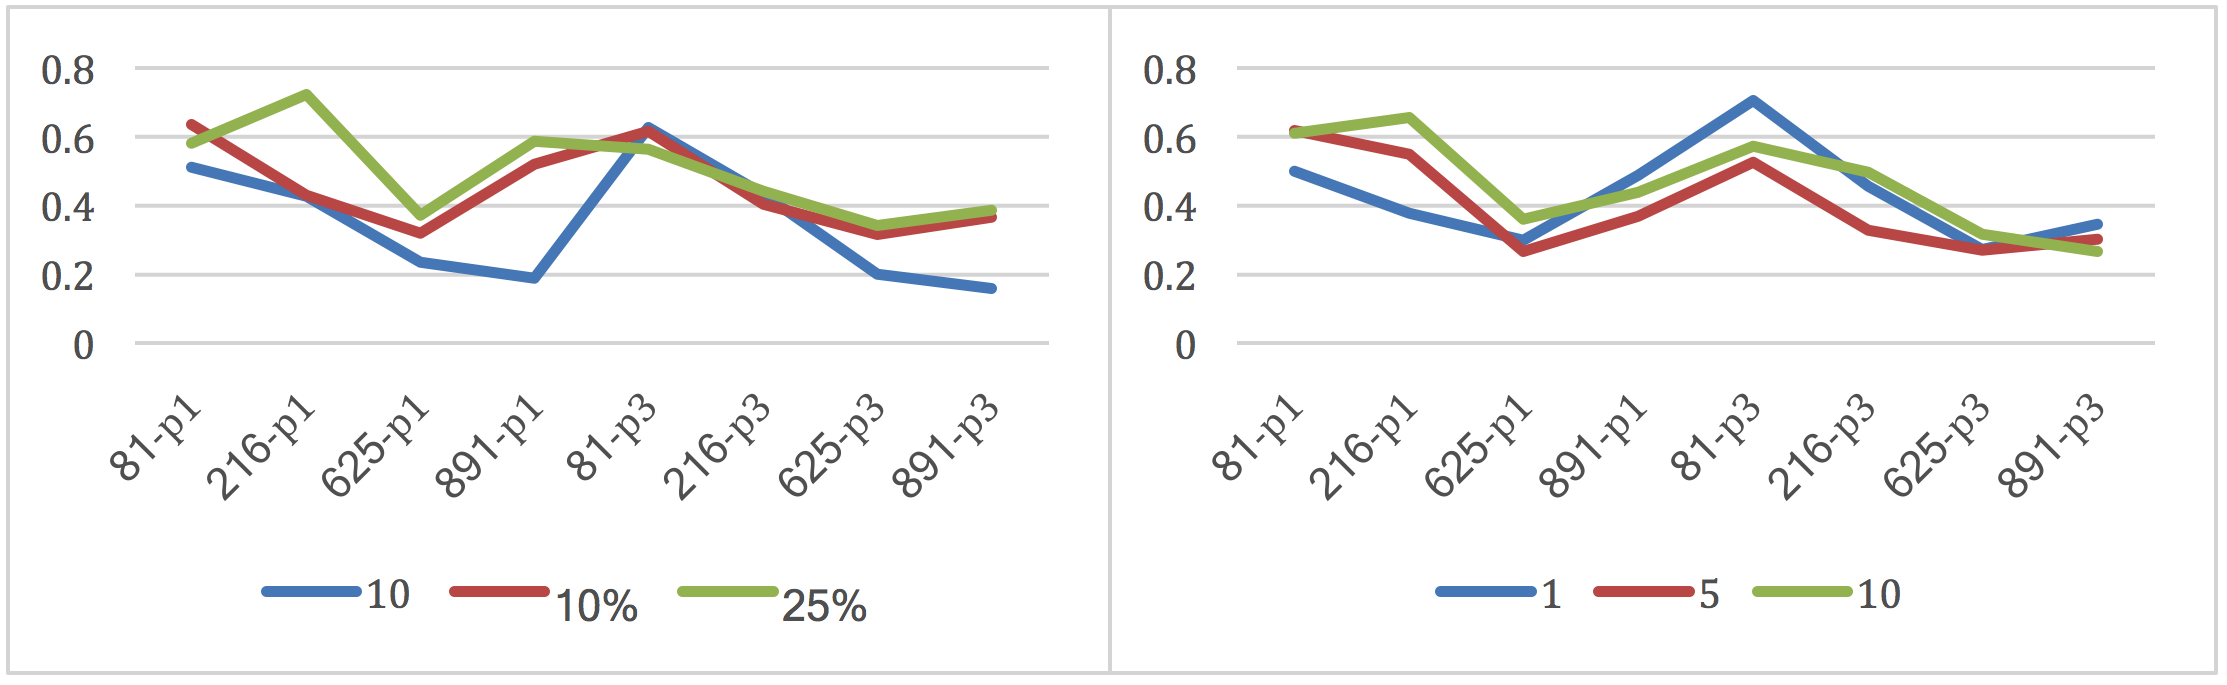
\includegraphics[width=1\textwidth]{figures/ga_accuracy}
	\caption{Accuracy of DSE, proportion of genetic NDS found in exhaustive NDS}
	\label{fig:acc_ga_ex}
\end{figure}
Figure~\ref{fig:gap_ga_ex} presents the generational distance results.  Here we find that the results are generally low, with the exception of the 891-point design space which is significantly worse, the reason for this is still to be determined.  The largest initial design space resulted in the lowest (best) values as did using a progress check condition value of five.


\begin{figure}[p]
	\centering
	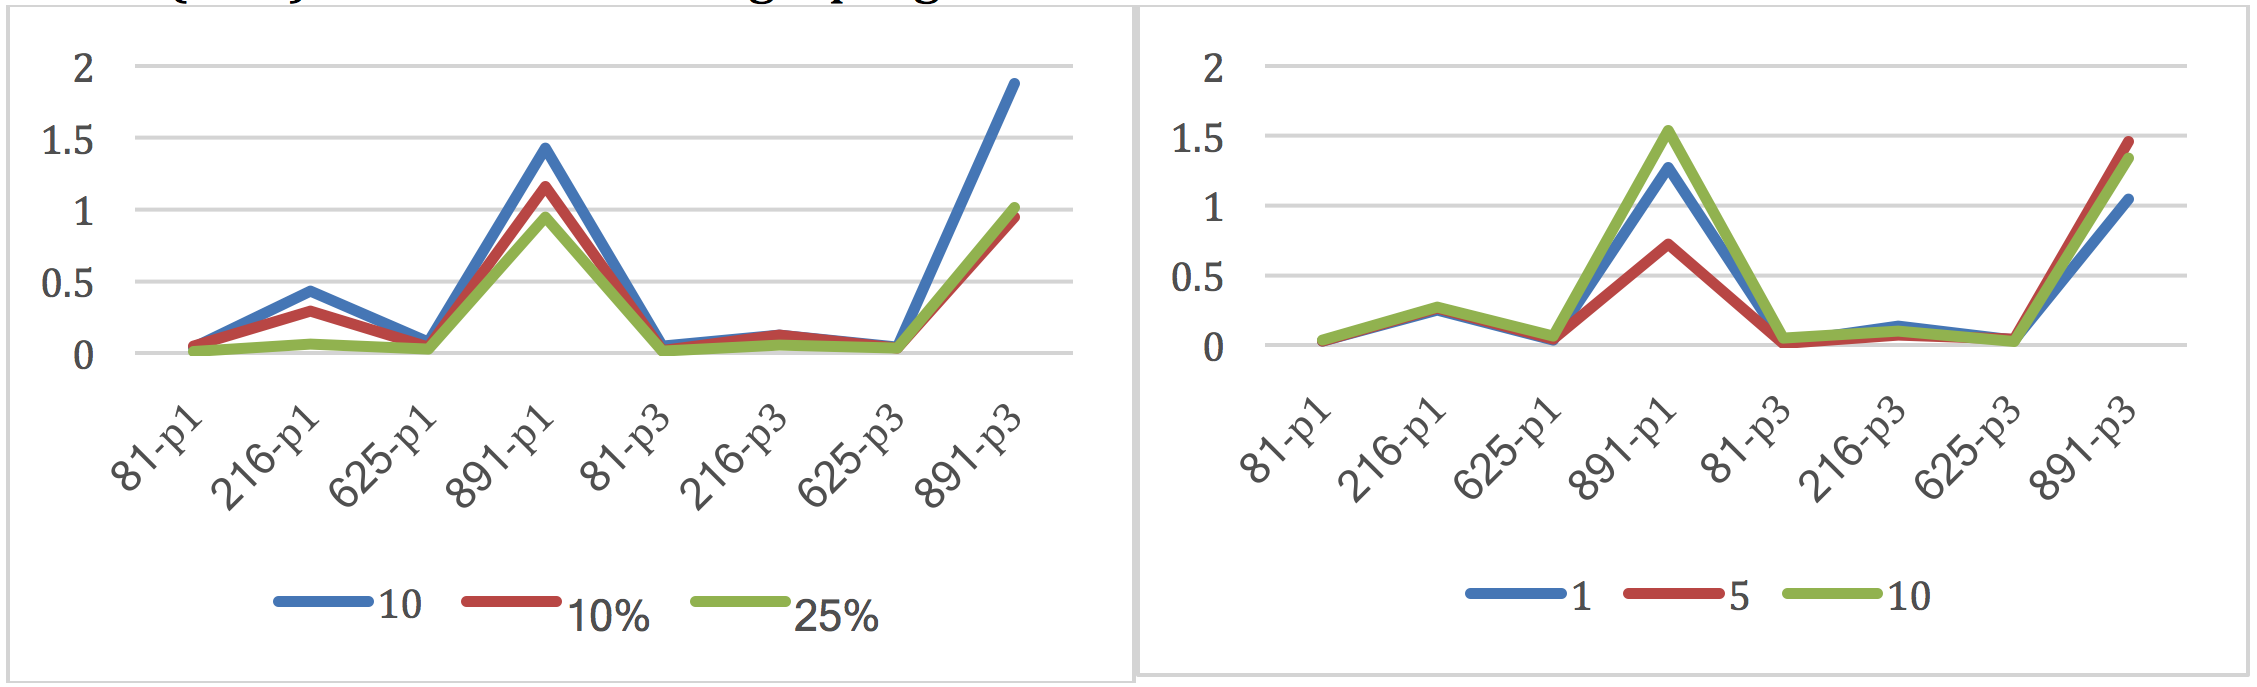
\includegraphics[width=1\textwidth]{figures/ga_distance}
	\caption{Gap between Genetic NDS and Exhaustive NDS}
	\label{fig:gap_ga_ex}
\end{figure}

\subsection{Selecting Approaches based on Design Space}

\draftnote{Editor: Carl Gamble}

\draftnote{CJG: Introduce what the user needs to consider.. number of designs, time to perform a simulation, simulations budget for the experiment (they may want more than one experiment performing)}

\draftnote{CJG: Basic rule, if you can perform exhaustive... do}

\draftnote{CJG: Increasing search resolution approach.}


\subsection{Cloud-Supported Design Space Exploration}

\draftnote{Editor: Carl Gamble}

\draftnote{CJG: The need for democratisation and how can HT Condor help}

\draftnote{CJG:  Basic working of Cloud based DSE, what is the process, how does it differ from local, how is it the same, where can the user find more.}

\draftnote{AI: Is there a unit on the y-axis that we should address (all graphs)}
